% ============================================================
% Chapitre 2 : Modele Statistique et Echantillonnage
% ============================================================
\chapter{Mod\`ele Statistique et \'Echantillonnage}
\label{ch:modele}

\begin{center}
\textit{<<~Tous les mod\`eles sont faux, certains sont utiles.~>>} --- George Box
\end{center}

% ------------------------------------------------------------
\section{Exemple motivant}
% ------------------------------------------------------------

Un laboratoire pharmaceutique teste un nouveau m\'edicament. Sur $n=100$ patients, 68 gu\'erissent. Le m\'edicament est-il efficace ? Pour r\'epondre, il faut un \emph{mod\`ele} : on suppose que chaque patient gu\'erit ind\'ependamment avec une probabilit\'e $p$ inconnue. Les 100 r\'esultats forment un \textbf{\'echantillon al\'eatoire} de loi $\mathcal{B}(1,p)$. Toute la statistique inf\'erentielle repose sur cette formalisation.

% ------------------------------------------------------------
\section{Mod\`ele statistique}
% ------------------------------------------------------------

\begin{definition}[Mod\`ele statistique]
\index{modele statistique@mod\`ele statistique}
Un \textbf{mod\`ele statistique} est un triplet $(\mathcal{X}, \mathcal{A}, \mathcal{P})$ o\`u :
\begin{itemize}
\item $\mathcal{X}$ est l'\textbf{espace des observations} (espace d'\'echantillonnage),
\item $\mathcal{A}$ est une tribu sur $\mathcal{X}$,
\item $\mathcal{P} = \{P_\theta : \theta\in\Theta\}$ est une famille de lois de probabilit\'e index\'ee par le \textbf{param\`etre} $\theta\in\Theta$.
\end{itemize}
\end{definition}

\begin{definition}[Mod\`ele param\'etrique vs.\ non param\'etrique]
\index{modele parametrique@mod\`ele param\'etrique}
\begin{itemize}
\item \textbf{Param\'etrique} : $\Theta\subseteq\R^d$ pour un $d$ fini. Exemple : $\mathcal{N}(\mu,\sigma^2)$, $\theta=(\mu,\sigma^2)\in\R\times\R_+^*$.
\item \textbf{Non param\'etrique} : $\Theta$ est de dimension infinie. Exemple : $\mathcal{P}$ = ensemble de toutes les lois continues sur $\R$.
\item \textbf{Semi-param\'etrique} : composante param\'etrique + composante non param\'etrique.
\end{itemize}
\end{definition}

\begin{definition}[Identifiabilit\'e]
\index{identifiabilite@identifiabilit\'e}
Le mod\`ele est \textbf{identifiable} si l'application $\theta\mapsto P_\theta$ est injective : $P_{\theta_1}=P_{\theta_2}\implies\theta_1=\theta_2$.
\end{definition}

% ------------------------------------------------------------
\section{\'Echantillon al\'eatoire}
% ------------------------------------------------------------

\begin{definition}[\'Echantillon al\'eatoire]
\index{echantillon aleatoire@\'echantillon al\'eatoire}
Un \textbf{\'echantillon al\'eatoire} de taille $n$ issu de la loi $P_\theta$ est un $n$-uplet $(X_1,\ldots,X_n)$ de variables al\'eatoires \textbf{ind\'ependantes et identiquement distribu\'ees} (i.i.d.) de loi $P_\theta$.

On note $X_1,\ldots,X_n \iid P_\theta$.

La \textbf{r\'ealisation} $(x_1,\ldots,x_n)$ est l'\'echantillon observ\'e.
\end{definition}

\begin{remarque}
La distinction entre $X_i$ (variable al\'eatoire) et $x_i$ (valeur observ\'ee) est fondamentale. Une \textbf{statistique} est une fonction des $X_i$ ; son \'evaluation en $(x_1,\ldots,x_n)$ donne une valeur num\'erique.
\end{remarque}

% ------------------------------------------------------------
\section{Statistiques et distributions d'\'echantillonnage}
% ------------------------------------------------------------

\begin{definition}[Statistique]
\index{statistique}
Une \textbf{statistique} est une fonction mesurable $T=T(X_1,\ldots,X_n)$ de l'\'echantillon qui ne d\'epend \emph{pas} du param\`etre $\theta$.
\end{definition}

\begin{definition}[Statistique exhaustive (suffisante)]
\index{statistique exhaustive}\index{statistique suffisante}
$T$ est \textbf{exhaustive} (ou suffisante) pour $\theta$ si la loi conditionnelle de $(X_1,\ldots,X_n)$ sachant $T$ ne d\'epend pas de $\theta$.
\end{definition}

\begin{theoreme}[Crit\`ere de factorisation de Fisher--Neyman]
\index{Fisher--Neyman}
\label{thm:fisher-neyman}
$T(X_1,\ldots,X_n)$ est exhaustive pour $\theta$ si et seulement s'il existe des fonctions $g$ et $h$ telles que :
\[
f(x_1,\ldots,x_n;\theta) = g\bigl(T(x_1,\ldots,x_n),\theta\bigr)\cdot h(x_1,\ldots,x_n),
\]
o\`u $f$ d\'esigne la densit\'e (ou la fonction de masse) jointe.
\end{theoreme}

\begin{proof}
\textit{(Cas discret.)} Si $T$ est exhaustive, $f(\mathbf{x};\theta) = P_\theta(T=T(\mathbf{x}))\cdot P(X=\mathbf{x}\mid T=T(\mathbf{x}))$. On pose $g(t,\theta)=P_\theta(T=t)$ et $h(\mathbf{x})=P(X=\mathbf{x}\mid T=T(\mathbf{x}))$.

R\'eciproquement, si la factorisation tient, alors :
\[
P_\theta(\mathbf{X}=\mathbf{x}\mid T=t) = \frac{g(t,\theta)\cdot h(\mathbf{x})}{\sum_{\mathbf{y}:T(\mathbf{y})=t} g(t,\theta)\cdot h(\mathbf{y})} = \frac{h(\mathbf{x})}{\sum_{\mathbf{y}:T(\mathbf{y})=t} h(\mathbf{y})},
\]
qui ne d\'epend pas de $\theta$.
\end{proof}

\begin{exemple}
Soit $X_1,\ldots,X_n\iid\mathcal{B}(1,p)$. La vraisemblance est :
\[
L(p) = \prod_{i=1}^n p^{x_i}(1-p)^{1-x_i} = p^{\sum x_i}(1-p)^{n-\sum x_i}.
\]
On identifie $g(t,p)=p^t(1-p)^{n-t}$ avec $t=\sum x_i$ et $h\equiv 1$. Donc $T=\sum X_i$ est exhaustive pour $p$.
\end{exemple}

% ------------------------------------------------------------
\section{Loi des grandes statistiques d'\'echantillonnage}
% ------------------------------------------------------------

\subsection{Moyenne empirique}

\begin{theoreme}[Esp\'erance et variance de $\xbar$]
Si $X_1,\ldots,X_n \iid$ avec $\E[X_i]=\mu$ et $\Var(X_i)=\sigma^2$, alors :
\[
\E[\xbar] = \mu, \qquad \Var(\xbar) = \frac{\sigma^2}{n}.
\]
\end{theoreme}

\begin{proof}
$\E[\xbar]=\frac{1}{n}\sum\E[X_i]=\mu$. Par ind\'ependance, $\Var(\xbar)=\frac{1}{n^2}\sum\Var(X_i)=\frac{\sigma^2}{n}$.
\end{proof}

\subsection{Loi des grands nombres}

\begin{theoreme}[Loi faible des grands nombres]
\index{loi des grands nombres}
Si $X_1,\ldots,X_n$ sont i.i.d.\ avec $\E[X_i]=\mu$ et $\Var(X_i)<\infty$, alors :
\[
\xbar \xrightarrow{\Prob} \mu \quad (n\to\infty).
\]
\end{theoreme}

\begin{theoreme}[Loi forte des grands nombres]
Sous les m\^emes hypoth\`eses (ou seulement $\E[|X_1|]<\infty$) :
\[
\xbar \xrightarrow{\text{p.s.}} \mu \quad (n\to\infty).
\]
\end{theoreme}

\subsection{Th\'eor\`eme central limite}

\begin{theoreme}[Th\'eor\`eme central limite (TCL)]
\index{theoreme central limite@th\'eor\`eme central limite}
\label{thm:tcl}
Si $X_1,\ldots,X_n$ sont i.i.d.\ avec $\E[X_i]=\mu$ et $0<\Var(X_i)=\sigma^2<\infty$, alors :
\[
\frac{\sqrt{n}(\xbar-\mu)}{\sigma} \xrightarrow{\mathcal{L}} \mathcal{N}(0,1).
\]
Autrement dit, $\xbar \approx \mathcal{N}\!\left(\mu,\frac{\sigma^2}{n}\right)$ pour $n$ grand.
\end{theoreme}

\begin{intuition}
Le TCL explique pourquoi la loi normale est omnipr\'esente : d\`es qu'une quantit\'e r\'esulte de la \textbf{somme de nombreux petits effets ind\'ependants}, elle est approximativement gaussienne.
\end{intuition}

\begin{center}
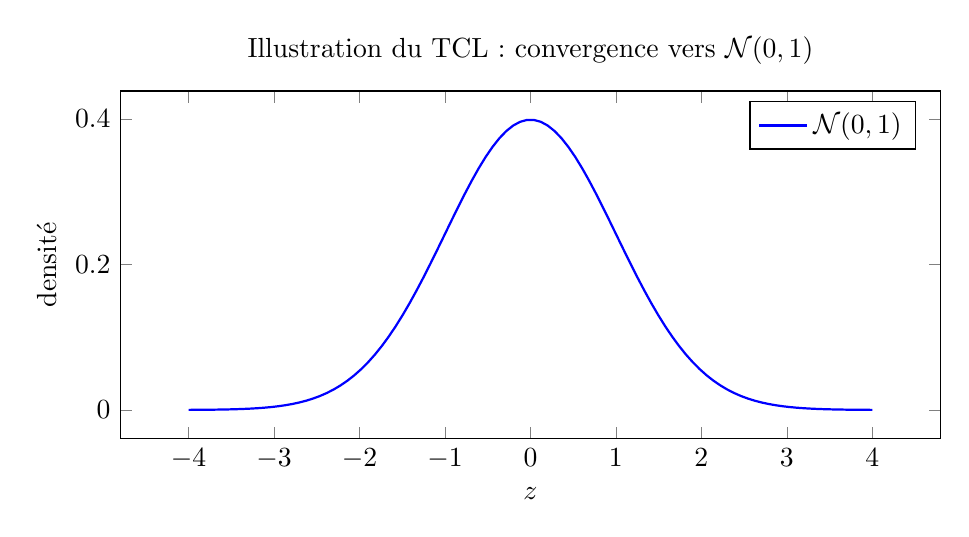
\begin{tikzpicture}
\begin{axis}[
    width=12cm, height=6cm,
    domain=-4:4, samples=100,
    xlabel={$z$}, ylabel={densit\'e},
    title={Illustration du TCL : convergence vers $\mathcal{N}(0,1)$},
    legend pos=north east
]
\addplot[thick,blue] {exp(-x^2/2)/sqrt(2*pi)};
\addlegendentry{$\mathcal{N}(0,1)$}
\end{axis}
\end{tikzpicture}
\end{center}

% ------------------------------------------------------------
\section{Distribution de la variance empirique}
% ------------------------------------------------------------

\begin{theoreme}[Loi de $S^2$ sous normalit\'e]
\label{thm:loi-s2}
Si $X_1,\ldots,X_n\iid\mathcal{N}(\mu,\sigma^2)$, alors :
\begin{enumerate}
\item $\xbar$ et $S^2$ sont \textbf{ind\'ependants} (th\'eor\`eme de Cochran),
\item $\displaystyle\frac{(n-1)S^2}{\sigma^2}\sim\chi^2(n-1)$.
\end{enumerate}
\end{theoreme}

\begin{corollaire}
Sous les hypoth\`eses du th\'eor\`eme~\ref{thm:loi-s2} :
\[
\frac{\xbar-\mu}{S/\sqrt{n}} \sim t(n-1).
\]
\end{corollaire}

\begin{proof}
On \'ecrit $\frac{\xbar-\mu}{S/\sqrt{n}} = \frac{(\xbar-\mu)/(\sigma/\sqrt{n})}{\sqrt{S^2/\sigma^2}} = \frac{Z}{\sqrt{V/(n-1)}}$ o\`u $Z\sim\mathcal{N}(0,1)$ et $V=(n-1)S^2/\sigma^2\sim\chi^2(n-1)$ sont ind\'ependants, donc le rapport suit $t(n-1)$ par d\'efinition de la loi de Student.
\end{proof}

% ------------------------------------------------------------
\section{Th\'eor\`eme de Glivenko--Cantelli}
% ------------------------------------------------------------

\begin{theoreme}[Glivenko--Cantelli]
\index{Glivenko--Cantelli}
Si $X_1,\ldots,X_n\iid F$, alors :
\[
\sup_{x\in\R}|\hat{F}_n(x)-F(x)| \xrightarrow{\text{p.s.}} 0.
\]
La fonction de r\'epartition empirique converge uniform\'ement vers la vraie fonction de r\'epartition.
\end{theoreme}

% ------------------------------------------------------------
\section{Impl\'ementation Python}
% ------------------------------------------------------------

\begin{python}
\begin{minted}{python}
import numpy as np
import matplotlib.pyplot as plt
from scipy import stats

# --- Illustration du TCL ---
np.random.seed(42)
n_values = [1, 2, 5, 30]
fig, axes = plt.subplots(1, 4, figsize=(16, 3.5))

for ax, n in zip(axes, n_values):
    means = [np.mean(np.random.exponential(1, n)) for _ in range(10000)]
    ax.hist(means, bins=40, density=True, alpha=0.7, edgecolor='black')
    ax.set_title(f"n = {n}")
    if n >= 5:
        x = np.linspace(min(means), max(means), 100)
        ax.plot(x, stats.norm.pdf(x, 1, 1/np.sqrt(n)), 'r-', lw=2)
plt.suptitle("TCL : moyennes d'exponentielles", fontsize=13)
plt.tight_layout()
plt.savefig("ch02_tcl.pdf")
plt.show()

# --- Glivenko-Cantelli ---
np.random.seed(0)
X = np.random.normal(0, 1, 50)
x_sorted = np.sort(X)
ecdf = np.arange(1, len(X)+1) / len(X)
x_grid = np.linspace(-3, 3, 200)

plt.figure(figsize=(8, 5))
plt.step(x_sorted, ecdf, where='post', label=r'$\hat{F}_{50}(x)$', lw=2)
plt.plot(x_grid, stats.norm.cdf(x_grid), 'r-', label=r'$\Phi(x)$', lw=2)
plt.legend()
plt.title("Glivenko-Cantelli : ECDF vs CDF normale")
plt.xlabel("x")
plt.ylabel("F(x)")
plt.savefig("ch02_glivenko.pdf")
plt.show()

# --- Statistique exhaustive : Bernoulli ---
n, p_true = 100, 0.68
sample = np.random.binomial(1, p_true, n)
T = sample.sum()
print(f"Statistique exhaustive T = sum(Xi) = {T}")
print(f"Estimation naturelle p_hat = T/n = {T/n:.2f}")
\end{minted}
\end{python}

% ------------------------------------------------------------
\section{Exercices}
% ------------------------------------------------------------

\begin{exercice}[$\star$ -- \'Echantillonnage]
On pr\'el\`eve un \'echantillon de taille $n=25$ d'une loi $\mathcal{N}(10,4)$. Calculer $\E[\xbar]$, $\Var(\xbar)$ et $\Prob(|\xbar-10|>0.5)$.
\end{exercice}

\begin{exercice}[$\star$ -- TCL en pratique]
G\'en\'erer 10\,000 moyennes d'\'echantillons de taille $n=30$ d'une loi $\mathcal{U}([0,1])$. V\'erifier graphiquement que la distribution est approximativement gaussienne. Calculer la moyenne et la variance empiriques et comparer aux valeurs th\'eoriques.
\end{exercice}

\begin{exercice}[$\star\star$ -- Exhaustivit\'e]
\begin{enumerate}
\item Soit $X_1,\ldots,X_n\iid\mathcal{P}(\lambda)$. Montrer que $T=\sum X_i$ est exhaustive pour $\lambda$.
\item Soit $X_1,\ldots,X_n\iid\mathcal{N}(\mu,\sigma^2)$ avec $\mu$ et $\sigma^2$ inconnus. Montrer que $T=(\sum X_i,\sum X_i^2)$ est exhaustive pour $(\mu,\sigma^2)$.
\end{enumerate}
\end{exercice}

\begin{exercice}[$\star\star$ -- Preuve du TCL par fonctions caract\'eristiques]
Soit $X_1,\ldots,X_n$ i.i.d.\ avec $\E[X_i]=0$, $\Var(X_i)=1$. On note $\varphi$ la fonction caract\'eristique de $X_1$.
\begin{enumerate}
\item Montrer que $\varphi(t)=1-\frac{t^2}{2}+o(t^2)$ au voisinage de 0.
\item Calculer la fonction caract\'eristique de $\bar{X}_n\sqrt{n}$.
\item En d\'eduire la convergence vers $\mathcal{N}(0,1)$.
\end{enumerate}
\end{exercice}

\begin{exercice}[$\star\star\star$ -- Projet : simulations Monte Carlo]
\'Etudier la vitesse de convergence du TCL pour diff\'erentes lois m\`eres (exponentielle, Bernoulli, uniforme, Cauchy). Pour chaque loi, estimer la taille $n$ minimale pour laquelle l'approximation normale est acceptable (test de Kolmogorov--Smirnov). Que se passe-t-il pour la loi de Cauchy ?
\end{exercice}

% ------------------------------------------------------------
\begin{formules}
\begin{align*}
\E[\xbar] &= \mu & \Var(\xbar) &= \sigma^2/n \\
\frac{\sqrt{n}(\xbar-\mu)}{\sigma} &\xrightarrow{\mathcal{L}} \mathcal{N}(0,1) &
\frac{(n-1)S^2}{\sigma^2} &\sim \chi^2(n-1) \\
\frac{\xbar-\mu}{S/\sqrt{n}} &\sim t(n-1) &
\sup_x|\hat{F}_n(x)-F(x)| &\xrightarrow{\text{p.s.}} 0
\end{align*}
Fisher--Neyman : $f(\mathbf{x};\theta) = g(T(\mathbf{x}),\theta)\cdot h(\mathbf{x}) \iff T$ exhaustive.
\end{formules}
